\documentclass[11pt,a4paper]{article}

% font
\renewcommand{\familydefault}{\sfdefault}


\usepackage[margin=0.8in]{geometry}
\usepackage[utf8]{inputenc}
\usepackage{amsmath}
\usepackage{amsfonts}
\usepackage{amssymb}

\usepackage[hidelinks]{hyperref}
\usepackage{float}

\usepackage{lipsum}% http://ctan.org/pkg/lipsum

%% Bibliography/references packages
\usepackage[comma]{natbib}
%%\bibliographystyle{agsm}
\bibliographystyle{dcu}

%% https://en.wikibooks.org/wiki/LaTeX/List_Structures
\usepackage{scrextend}

% tables, row colour
\usepackage{tabularx,colortbl}
% For vertical centering text in X column
\renewcommand\tabularxcolumn[1]{m{#1}}

% https://tex.stackexchange.com/questions/22751/how-to-force-table-caption-on-top
%\usepackage[tableposition=top]{caption}
\usepackage{float}
\floatstyle{plaintop}
\restylefloat{table}

% https://en.wikibooks.org/wiki/LaTeX/List_Structures
\usepackage{enumitem}

% https://jansoehlke.com/2010/06/strikethrough-in-latex/
\usepackage{ulem}


%% Report variables
\newcommand{\scname}{PRCO304}
\newcommand{\dlatestv}{1.00}

\definecolor{babyblueeyes}{rgb}{0.63, 0.79, 0.95}
\definecolor{ballblue}{rgb}{0.13, 0.67, 0.8}
\definecolor{beaublue}{rgb}{0.74, 0.83, 0.9}

\usepackage{array,booktabs,arydshln,xcolor}
\usepackage{xcolor}% http://ctan.org/pkg/xcolor
\usepackage{fancyhdr}% http://ctan.org/pkg/fancyhdr
\fancypagestyle{main}{%
	\renewcommand{\headrulewidth}{2pt}
	\renewcommand{\headrule}{\hbox to\headwidth{%
		\color{babyblueeyes}\leaders\hrule height \headrulewidth\hfill}}
	\renewcommand{\footrulewidth}{2pt}
	\renewcommand{\footrule}{\hbox to\headwidth{%
		\color{babyblueeyes}\leaders\hrule height \headrulewidth\hfill}}
	
	%\fancyhf{}
	%\fancyhead[LE]{\textbf{\leftmark}}
	%\fancyhead[RE]{\textbf{\scname{}}}
	%\fancyhead[LO]{\textbf{\scname{}}}
	%\fancyhead[RO]{\textbf{\rightmark}}

	%\fancyfoot[LE]{\textbf{\thepage}}
	%\fancyfoot[RE]{\textbf{\scname{} Configuration Guide}}
	%\fancyfoot[LO]{\textbf{\scname{} Configuration Guide}}
	%\fancyfoot[RO]{\textbf{\thepage}}
}


%% Make bibliography show in table of contents
%% https://tex.stackexchange.com/questions/8458/making-the-bibliography-appear-in-the-table-of-contents
\usepackage[nottoc,numbib]{tocbibind}
%% ^^^ overwrites \bibname, so set it back
\renewcommand{\bibname}{References}

\RequirePackage{filecontents}
\begin{filecontents}{prco304_h4.bib}
@inproceedings{safety_fpga,
  title={FPGAs in critical hardware/software systems},
  author={Hilton, Adrian J and Townson, Gemma and Hall, Jon G},
  booktitle={Proceedings of the 2003 ACM/SIGDA eleventh international symposium on Field programmable gate arrays},
  pages={244--244},
  year={2003},
  organization={ACM}
}
@online{defstan_0056,
	title={Safety Management Requirements for Defence Systems},
	url={https://segoldmine.ppi-int.com/content/standard-def-stan-00-56-safety-management-requirements-defence-systems},
	year={2007}
}
@article{defstan_0056_2,
  title={Safety-critical systems, formal methods and standards},
  author={Bowen, Jonathan and Stavridou, Victoria},
  journal={Software Engineering Journal},
  volume={8},
  number={4},
  pages={189--209},
  year={1993},
  publisher={IET}
}
@article{iec61508,
  title={Introduction to IEC 61508},
  author={Bell, Ron},
  booktitle={Proceedings of the 10th Australian workshop on Safety critical systems and software-Volume 55},
  pages={3--12},
  year={2006},
  organization={Australian Computer Society, Inc.}
}

@misc{scarabhardware,
title={MiniSpartan6+}, 
journal={{Scarab Hardware}},
url={https://www.scarabhardware.com/minispartan6/},
year=2014
}
@misc{arty,
title={Arty Artix-7 FPGA Development Board}, 
journal={{Avnet}},
url={https://uk.rs-online.com/web/p/programmable-logic-development-kits/1346478/},
year=2015
}
@misc{arndt2002algorithms,
  title={Algorithms For Programmers},
  author={Arndt, J{\"o}rg},
  year = 2002
}
@book{hdl,
title={HDL Programming Fundamentals: VHDL and Verilog},
author={Nazeih Botros},
year={2006},
publisher={Da Vinci Engineering Press}
}

@misc{arm, title={ARM in the World of FPGA-Based Prototyping}, url={https://community.arm.com/processors/b/blog/posts/arm-in-the-world-of-fpga-based-prototyping}, journal={Arm Community},
year={2016}}

@book{microblaze,
title={MicroBlaze 
Processor Reference 
Guide},
journal={Xilinx},
year={2017}
} 

\end{filecontents}

%s comments
\usepackage{verbatim}

%inline graphs
\usepackage{wrapfig}
% multiple figures on line
\usepackage{subfig}

\usepackage{graphicx}
\graphicspath{ {img/} }

% Caption font size
% https://tex.stackexchange.com/questions/86120/font-size-of-figure-caption-header
\usepackage[font=scriptsize,labelfont=bf]{caption}

%\setlength{\belowcaptionskip}{-10pt}
%\setlength{\abovecaptionskip}{-5pt} % Chosen fairly arbitrarily


\usepackage{fancyhdr}
\pagestyle{fancy}
\lhead{\rightmark}
\chead{}
%\rhead{FPGA-based RISC Microprocessor and Compiler (Rev. \dlatestv{})}
\rhead{PRCO304 (Rev. \dlatestv{})}
\lfoot{Ben Lancaster 10424877}
\cfoot{}
\rfoot{Page \thepage}

\renewcommand{\subsectionmark}[1]{\markright{\thesubsection\ #1}}


\begin{document}

\makeatletter
\DeclareRobustCommand*{\nameref}{%
\color{blue}%
        \@ifstar\T@nameref\T@nameref
        }%
\makeatother

\begin{titlepage}
\begin{center}

\vspace*{5cm}
\Large
\textbf{
%%PRCO304 - Project Initiation Document
%Highlight Reports
FPGA-based RISC Microprocessor and Compiler (Rev. \dlatestv{})
}

\vspace{0.4cm}
\large
%%Space optimised FPGA-based side-microprocessor.
PRCO304 - Final Stage Computing Project
%%EMBEDDED CPU - FPGA-based RISC microprocessor

\vspace{4cm}
\textbf{Ben Lancaster 10424877}\\
\today 


\end{center}

\end{titlepage}

\pagestyle{main}

\section*{Revision History}
\begin{table}[h]
\def\arraystretch{1.5}%  1 is the default, change whatever you need
    \begin{tabularx}{\textwidth}{|l|l|X|}
    \hline
    Date & Version & Changes \\
	\specialrule{2pt}{-2pt}{0pt}
	11/03/2018 & 1 & Initial section outline. \\ \hline
    \end{tabularx}
    \caption{Document revisions.}
\end{table}
\newpage


\section*{Abstract}
ben

\newpage
\renewcommand*\contentsname{Table of Contents}
\tableofcontents
\listoffigures
\listoftables
 
\newpage

\section{Introduction}

\section{Background}
\subsection{Current Implementations}

\section{Objectives}

\newpage
\section{Legal and Ethical Considerations}
\subsection{Privacy}
The \scname{} processor will be able to read and write to all data passing through it and control all connected peripherals (such as UARTs, SDRAMs, and SD Cards). The processor does not track or store usage behaviour, instructions and their frequency,   memory contents, or timing statistics, or any other usage metric.

\subsection{Fit for Purpose}
The \scname{} processor is not designed to run general purpose operating systems, such as Linux or embedded RTOS systems. All memory devices attached to the FPGA are fully accessible to the processor core and instructions/programs running through it, meaning that operating systems or secure applications storing private and sensitive information is not protected by modern processor features such as privilege modes and virtual memory sections. The processor lacks common components required to run modern operating systems, such as a memory management unit (MMU) and privilege modes, and so should not be run on the processor.

The \scname{} processor is not designed to run in high-reliability or safety-critical environments that require established safety standards, such as the UK Defence Standard 00-56 \citep{defstan_0056_2} and IEC 61508 \citep{iec61508}.

The \scname{} processor, by design, should be used as a replacement for a simple micro-controller accompanying a main processing module.

\subsection{Third-party Libraries}
This project uses only 1 external library for the processor core's universal asynchronous receiver-transmitter (UART) module that does not depend on any other libraries. This allows me to guarantee that: the project rights are secure; and application behaviour is well-defined and predictable (no exploits introduced/injected from external libraries). The UART module does feature a large first-in-first-out (FIFO) buffer for temporary storage of in- and out- going messages. This FIFO is internal to the FPGA design and so is protected from external viewing/modification by probing the board in which the core is running on.

The compiler sub-project does not use any external library dependencies, does not record telemetry or usage statistics, and does not require an internet connection to run.

\subsection{Generated Code}
The code generated by the compiler is \textbf{not guaranteed} to:
\begin{itemize}
\item{\textbf{produce constant time executable code for expressions}. For example, the compiler output for an \textit{if} statement may implicitly vary depending on the it's, which may have been optimised out, constant-folded, or without-optimisation. This also applies for user code aiming to create reliable and accurate time delay loops; although the processor does not perform optimisations such as instruction caching or branch prediction, access to memory and ALU operations may vary in time.}
\item{\textbf{produce code for secure-environments}. The compiler will not randomise, obfuscate, or split-up and spread, output code. Output machine code will be in a predictable format (global variables in low-memory, instruction memory in middle-memory, and stack memory in high-memory) making the binary easily subject to reverse-engineering and modification.}
\end{itemize}


\section{Project Management}

\section{Requirements}

\newpage
\section{High Level Design}

\begin{figure}[H]
\begin{center}
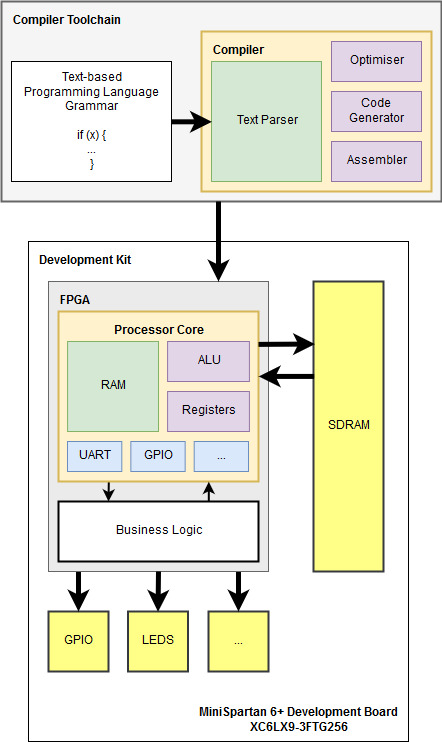
\includegraphics[scale=0.39]{hld}
\end{center}
\caption{test}
\label{fig:hld}
\end{figure}

\subsection{Registers}
\subsection{Pipeline Architecture}


\section{Testing and Verification}

\section{Conclusion}

\section{Appendices}
\subsection{Appendix A. PRCO Core Reference Guide}
\subsection{Appendix B. PRCO Compiler Reference Guide}
\subsection{Appendix C. Project Initiation Document}

\newpage
\bibliography{prco304_h4} 
\end{document}